\chapter{Requirements Engineering} % Main chapter title
\label{chap:Requirements_Engineering}
This chapter has the purpose to present the process in which the requirements, both functional and non-functional, were gathered. It will start with an overview over the existent user groups, and then presenting the functional requirements. 

\section{User Groups}
\label{sec:Requirements_userGroups}
In this section, the existent actors and their actions will be presented. This will provide a better understanding regarding the users and their responsibilities in the platform.
\par

\begin{figure}[ht]
\centering
\begin{minipage}{.5\textwidth}
  \centering
  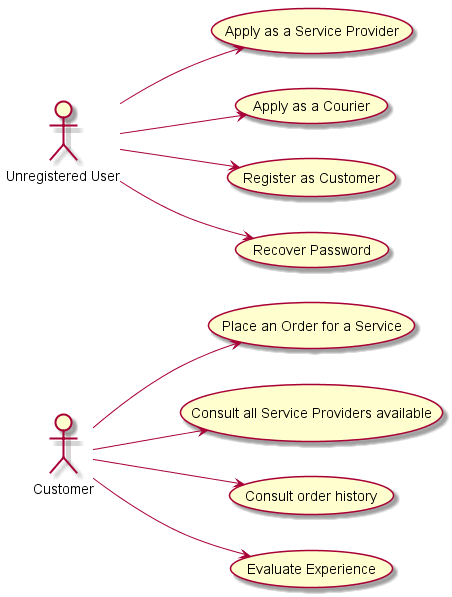
\includegraphics[width=\linewidth]{chapters/Requirements_Engineering/assets/FrontOfficeUseCaseDiagram.png}
\end{minipage}%
\begin{minipage}{.5\textwidth}
  \centering
  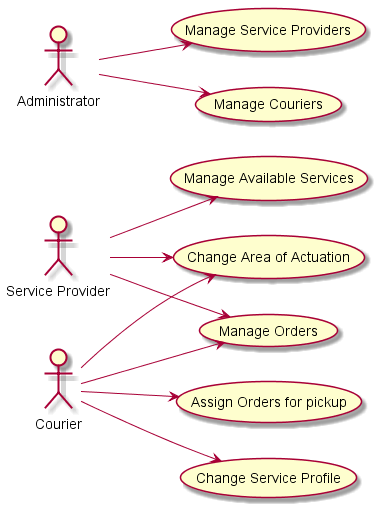
\includegraphics[width=\linewidth]{chapters/Requirements_Engineering/assets/BackOfficeUseCaseDiagram.png}
\end{minipage}
\caption[Use Case Diagram]{Use Case diagram}
\label{fig:useCaseDiagram}
\end{figure}

\par

Considering that there will be different responsibilities for the users of this platform, there is a need to define what are they and which user groups do the define. Hereupon, the main users of the platform will be:

\begin{itemize}
    \item \textbf{Unregistered User} - A user who has just reached the platform. Hasn't authenticated yet;
    \item \textbf{Customer} - A user which is a customer and is in look of a service;
    \item \textbf{Courier} - A user which is a courier and will be the people which will make the transportation of the necessary goods and materials associated to a service;
    \item \textbf{Service Provider} - A user which is a service provider and will be the responsible to provide the service requested by the customer;
    \item \textbf{Administrator} - The administrator of the platform. Responsible to manage service providers, couriers and the platform as a whole. 
\end{itemize}
\par


\par
The figure \ref{fig:useCaseDiagram} presents a use case diagram where it is possible to see all the actors and the functionalities that each one can access. On the left side there are the actors which access the core front-office functionalities such as placing an order or register. These actors are the customer and an unregistered user. On the right side we have the management and back-office actors that are responsible for the operational side of the platform. The actors for these actions are the service provider, the courier and the platform administrator.

\section{Functional Requirements}
\label{sec:functional-requirements}
In this section, the functional requirements of the system will be presented. Each of the requirements will then be split in smaller user stories throughout the project.

\subsection{FF01 - Register as Customer}
\textbf{User Groups}: Unregistered User

\subsubsection{Requirement Description}
Besides being able to consult some marketing material and information about the platform, the most common action that an unregistered user can make is registering. If the user chooses to register as a customer, some data will be needed to make it happen. The mandatory information for the registration be successful are: 
\begin{itemize}
    \item Name
    \item E-Mail
    \item Password
\end{itemize}

The user may complement with other information (address, phone contact, edit information) in the “My account” page.
\par
After the registration, an email will be sent to confirm the email address. In that email, there will be an url for the confirmation. While the account has not been activated, no orders may be done.


\subsection{FF02 - Apply as a Service Provider}
\textbf{User Groups}: Unregistered User

\subsubsection{Requirement Description}
An unregistered user may also choose to apply as a service provider. In this case, some data will be needed to make it happen. The mandatory information for the registration be successful are: 
\begin{itemize}
    \item Name of the service provider
    \item Name of the representative
    \item Address
    \item Service type (Laundry, mechanics, warranty...)
    \item Area of Actuation (Coordinates of the location of the service provider and the desired radius)
    \item Email
    \item Password
\end{itemize}

The user may complement with other information (phone contact, edit information) in the “My account” page.
\par
After the registration, this application for service provider will be sent to the platform administrators which will evaluate the viability of the \gls{SP}. In a first version, the management of the applications for service provider is not in the scope of this project. 
\par
The service provider will only be available in the platform after the administrator’s approval.

\subsection{FF03 - Apply as a Courier}
\textbf{User Groups}: Unregistered User

\subsubsection{Requirement Description}
An unregistered user may also choose to apply as a courier. In this case, some data will be needed to make it happen. The mandatory information for the registration be successful are: 
\begin{itemize}
    \item Name
    \item Profile type (motorcycle, van, car, etc.)
    \item Area of Actuation
    \item Email
    \item Password
\end{itemize}

\par
After the registration, this application for courier will be sent to the platform administrators which will evaluate the viability of the courier. In a first version, the management of the applications for courier is not in the scope of this project. 
\par
The courier will only be available in the platform after the administrator’s approval.



\subsection{FF04 - Log In}
\textbf{User Groups}: Unregistered User

\subsubsection{Requirement Description}
In order to authenticate before the platform, the unregistered user needs to log into an account. This is done with the email and password set upon the registration. If the password was changed after the registration, the latest password must be used.

\subsection{FF05 - Recover Password}
\textbf{User Groups}: Unregistered User

\subsubsection{Requirement Description}
In case of a lost/stolen password, an user may request for a password restore. To do this, the user must provide the email associated to the account and an email will be sent with a link to restore the password.

\subsection{FF06 - Place an order for a service}
\textbf{User Groups}: Customer

\subsubsection{Requirement Description}
When a customer selects a service that he/she desires, it will trigger the main process of the platform. Starting on the \gls{SDP}, the user needs to input some information regarding the service itself (in case of laundry, the platform will need information about the size of the size of the article, among others). After filling up all information regarding the selected service, the customer will be taken to the checkout page. In the checkout page, the customer will need to fill more information:
\begin{itemize}
    \item Pickup address
    \item Delivery address
    \item Billing address
    \item Preferred pickup hours
    \item Preferred delivery hours
\end{itemize}

After filling up all the information, the customer will be led to the payment page where he/she will select one of the existing payment options. This process will be done by a third party.
\par 
When the payment is completed, the order will be registered in back-office, an email with the order confirmation will be sent to the customer, and the order will be available to be consulted to the customer, the service provider that was selected and the couriers, to assign the orders.
At this point, the customer also needs to print the shipping guide, that will follow the article to the article.


\subsection{FF07 - Check all available service providers}
\textbf{User Groups}: Customers, Unregistered User

\subsubsection{Requirement Description}
When entering the platform web page, the customer (registered or not) will be able to check all the existing service providers and their services. All the services will be presented under its service provider on the \gls{SLP}. On this page, only basic information will be shown, as a description of the service and an estimate of prices.

\subsection{FF08 - Check order history}
\textbf{User Groups}: Customers

\subsubsection{Requirement Description}
The customer will be able to check their order history. This menu will be available as a tab of the “My Account” page.
\par
This page will show all orders made, date, and status (check section \ref{sub:order-states} for more information regarding the order states). The customer can also open the orders to get more information of what was ordered.


\subsection{FF09 - Evaluate Experience}
\textbf{User Groups}: Customers

\subsubsection{Requirement Description}
Every service provider will have a rating, depending on the performance for each service. This rating will be made by the customer after each order. The customer will need to rate some aspects regarding their experience with the platform, the service provider and the courier. In the first version, only service providers will have a rating. The customer will need to answer questions (classify 0-10) as:
\begin{itemize}
    \item How was your experience regarding the order process?
    \item Did the Service Provider fulfill your expectations?
    \item What about the experience with the courier?
\end{itemize}

\subsection{FF10 - Manage available services}
\textbf{User Groups}: Service Providers

\subsubsection{Requirement Description}
As the platform's service providers’ business grows, so will grow the offering of services available. This menu allows the service providers to create new, change and delete existent services. To be noted that a change of a service will actually create a new one, in order for the current orders for that service don't be changed.

\subsection{FF11 - Manage orders}
\textbf{User Groups}: Service Providers, Couriers

\subsubsection{Requirement Description}
In this menu, the service provider will be able to check all orders (current and past) and move them between a series of steps:
\begin{enumerate}
    \item New
    \item Picked on customer address
    \item Delivered to Service Provider
    \item Service Started
    \item Service Finished
    \item Picked on Service Provider Address
    \item Delivered to Customer
    \item Canceled
\end{enumerate}

The section \ref{sub:order-states} provides further information regarding the order states and its transitions.
\par
If the shipping guide is lost for some reason, the service provider can also print that document.

\clearpage
\subsection{FF12 - Change Area of Actuation}
\textbf{User Groups}: Service Providers, Couriers

\subsubsection{Requirement Description}
Both the couriers and service providers will need to select the \gls{AoA}. Only customers within this area of actuation will be able to select the services of the service provider in question. Likewise, couriers also need to select an area where they can make transportation. For an order to be fulfilled, there needs to be a courier that has both the customer and the service provider in their \gls{AoA}.

\subsection{FF13 - Change service profile}
\textbf{User Groups}: Couriers

\subsubsection{Requirement Description}
There may be services that require different kinds of vehicle for the goods to be transported. In this menu, the courier can change his vehicle type. There will be three options:
\begin{itemize}
    \item Scooter
    \item Car
    \item Van
\end{itemize}

In this case, a Van can transport any kind of goods, and a scooter will only be able to transport small goods.


\subsection{FF14 - Assign orders for pickup}
\textbf{User Groups}: Couriers

\subsubsection{Requirement Description}
The courier will be presented all the unassigned orders of in the defined \gls{AoA}. Here, the courier will be able to assign himself to the orders, meaning that he/she accepts to make the transportation and picking up the goods the schedule requested by the customer. When this assign is done, an email notification is sent to the courier’s email and the customer as well.

\clearpage
\subsection{FF15 - Manage Service Providers}
\textbf{User Groups}: Administrators

\subsubsection{Requirement Description}
In this menu, the platform administrators will be able to create, remove and consult information about the existing Service Providers.

\subsection{FF16 - Manage Couriers}
\textbf{User Groups}: Administrators

\subsubsection{Requirement Description}
In this menu, the platform administrators will be able to create, remove and consult information about the existing Couriers.

\section{Non-Functional Requirements}
\label{sec:non-functional-requirements}
In the previous section, the functional requirements were identified. Those requirements help to understand \textbf{what} the application will do. On the other hand, non-functional requirements specify \textbf{how} the application will do it. 
\par
In this section, an overview will be given regarding these requirements. They are to be considered throughout the development of the features identified in the section \ref{sec:functional-requirements}.

\subsection{Usability}
The system needs to be accessible from anywhere. This means that web apps need to be responsive for users being able to access it from mobile devices.

\subsection{Security}

The SnapTasks Portal is the one which will be responsible for managing the order requests and by consequence, it will also be responsible for managing the payments. It is mandatory to ensure the security of the payments, to diminish fraudulent orders. 
\par
To avoid man-in-the-middle attacks, all communications between services must be done using HTTPS.
\par
All personal data must be handled taking into account the current legislation.
\par
The system as a whole must have, at least, basic security systems, as:
\begin{itemize}
    \item \textbf{Authentication:} the system must be sure of who is making a certain request. This can be managed using username/password login;
    \item \textbf{Authorization:} the system must ensure that whoever is making a certain request, has permissions to do so. This can be managed by assigning roles to users, where a role grants access to a number of functionalities.
\end{itemize}

\subsection{Availability}
The SnapTasks Portal must have the minimum downtime possible, for not losing customers because of having the website down.
The back-office tools should also be down the least time possible. However, this scenario has a lighter impact, since the customers are still able to access the portal and place orders.

\subsection{Scalability}
The delivered solution must be capable to be scaled dynamically. This means that the access of many different users at the same time does not affect the website performance. 
\par
To attain this, a cloud service, such as \textit{Azure} is to be used, allowing to increase and decrease the hardware resources depending on the needs.

\subsection{Resilience}
The platform must be resilient to handle wrong input from the users or sudden failures of dependent services. 
\par 
Those errors should be handled and the user who has made the request should be informed about what happened. 

\subsection{Performance}
The system must be fast and efficient in order not to lose a customer because the application was not responding. For this to happen, most of the processing should be done in back-office, using asynchronous processes.
\par
This requirement will be more important as the platform has more users. 

\par

\subsection{Internationalization and Localization}
The platform will be used firstly in Portugal, therefore, it should have its front-office in Portuguese.
\par
However, as the platform grows, there may be the need to have SnapTasks Portal in different languages and cultures. The application should be prepared for that case.

\subsection{Maintainability}
The platform code should be easy to maintain. This means that both bug fixing and adding new features should be as easy as possible, following the industry's best practices.

\section{Process View}
To have a better understanding of how the whole platform will work, we need to have a clear view of the operational process which this system supports. This can be achieved by analyzing the flow that an order takes, since it is placed until the service is finished and all goods are returned to the customer.
\par
It starts when a registered customer accesses the system. He/she will select a service he/she needs, proceed to checkout, make the payment and place the order. At this point, the order is created in the system and can be accessed by the courier to assign himself, compromising to make the delivery from the customer's pickup address to the service provider address. This assignment is only for the first leg of this order (from the customer to the \gls{SP}). At the date selected by the customer, the courier will go to the customer's address to pickup the goods associated to the order and then deliver them to the service provider. The service provider now has the goods and is ready perform the ordered service. After the service is finished, the order status is changed to \textit{Service Finished}, allowing the couriers to know that the goods associated to that order are ready to be returned to the customer. Therefore, they also can assign themselves to that transportation, compromising that they will do the second leg of the order (from the \gls{SP} to the customer). In this case, the goods can be picked up at any time, because the service provider has an open store. After picking up the goods at the \gls{SP}'s address, the courier will deliver the items to the customer, finishing the process.
\par

The figure \ref{fig:processDiagram} presents a more graphical view of this process and shows how the user groups interact.

\begin{figure}[ht]
\centering
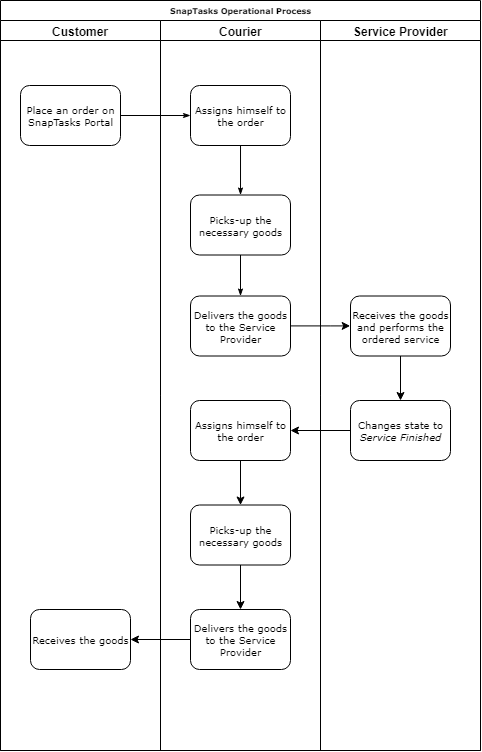
\includegraphics[width=0.98\textwidth,keepaspectratio]{chapters/Requirements_Engineering/assets/ProcessDiagram.png}
\caption[Process diagram]{Process diagram}
\label{fig:processDiagram}
\end{figure}

\clearpage

\section{Order Process States}
\label{sub:order-states}

In the previous section, it was possible to understand that the order goes through several steps for the service to be fulfilled. These steps are represented by the states in which an order can be.
Each state represents something that is occurring/occurred, or an action that is needed.
\par
The possible states for a given order are the following:

\begin{itemize}
    \item New;
    \item Picked on customer address;
    \item Delivered to Service Provider;
    \item Service Started;
    \item Service Finished;
    \item Picked on Service Provider Address;
    \item Delivered to Customer;
    \item Canceled.
\end{itemize}

These states reflect the operational status. Each order must go through these states sequentially. For example, an order cannot be delivered to the customer before the service is finished, or, an order's service cannot start before the goods are delivered to the service provider.
\par
The figure \ref{fig:orderStateDiagram} shows how the order states connect to each other and represents the happy path workflow.

\begin{figure}[ht]
\centering
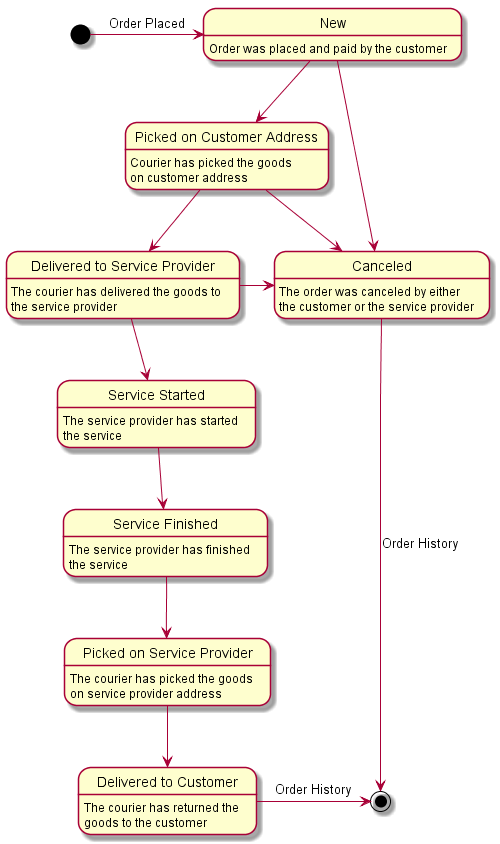
\includegraphics[width=0.91\textwidth,keepaspectratio]{chapters/Requirements_Engineering/assets/StateDiagram.png}
\caption[Order State diagram]{Order State diagram}
\label{fig:orderStateDiagram}
\end{figure}
